\section{Methods}\label{sec:methods}

\subsection{Model}

As the object of our interpretation technique, we chose a pretrained BERT model, short for Bidirectional Encoder Representations from Transformers \citep{devlin_bert_nodate}. For completeness, BERT is a transformer model which maps a set of subword tokens to another set of such tokens. BERT has been originally trained on two different natural language processing objectives. First, it has been tasked with a masked language modeling (MLM) objective. This refers to the task of reconstructing a short input text which has been intentionally corrupted. The corruption typically consists in eliminating (i.e. masking) a random proportion of the tokens contained in the input text (e.g. "BERT is a transformer model." might be corrupted as "BERT is a [MASK] model."). Given this, the MLM task consists in reconstructing the pre-corruption text from the corrupted version.

The second objective employed in training BERT is a next sentence prediction (NSP) task. Given a pair of two sentences, BERT is tasked with predicting whether they are consecutive in the original text. The combination of those two conceptually simple objectives has been shown to help BERT learn rich semantic representations of the text being processed, as an instrumental goal in solving the two tasks. For instance, mean-pooling token embeddings across texts has been shown to be highly effective in downstream information retrieval tasks based on vector similarity \citep{reimers_sentence-bert_2019}. Moreover, mean-pooling token embeddings of a text and comparing the result with the mean-pooled embeddings of a set of labels (e.g. science, politics, economics), has been shown to be a competitive baseline in text classification \citep{yin_benchmarking_2019}. Alternatively, BERT models fine-tuned on limited data from other tasks (e.g. natural language inference) had yielded state-of-the-art performance in multiple tasks \citep{jiang_evaluating_2019}.

Internally, BERT represents each token as an embedding of dimensionality 768. As the model consists of a repetitive sequence of layers, the set of embeddings which represents tokens is adjusted from one layer to the next using multi-head attention mechanisms. It is precisely those token embeddings which we are trying to distill knowledge graphs from using the NSC approach. Specifically, as often done in the mentioned applications, we are attempting to interpret the set of embeddings which are generated in the \textit{last} BERT layer. This has been hypothesized to contain high-level features extracted the input tokens which are based in large part on the tokens' contexts, after extensive processing in the earlier layers of the model \citep{tenney_bert_2019}.

We opted for BERT due to its widespread use in industry applications and its large number of derivative models (e.g. RoBERTa \citep{liu_roberta_2019}, ALBERT \citep{lan_albert_2020}, distilBERT \citep{sanh_distilbert_2020}, DeBERTa \citep{he_deberta_2021}, etc.). As mentioned before, BERT takes in a sequence of subword tokens as input and reconstructs it as output, while generating a unique contextual embedding for each token. Crucially, the same token can be attributed different embeddings in different contexts (e.g. "she" referring to different people). In practice, the contextual embeddings of individual tokens are mean-pooled together to yield an overarching document embedding. However, here we focus only on the contextual embeddings of \textit{individual} tokens or at most short sequences of them which form a noun phrase (e.g. "orange juice").

\subsection{Data}

As NSC requires an auxiliary dataset for generating state clouds of contextual embeddings, we employ one of the datasets which have been used for training the BERT model, namely BookCorpus \citep{devlin_bert_nodate}. This dataset consists of a variety of public domain books across different genres, and provides many different contexts for symbols to appear in as exemplars.

We focus our investigation on relating a set of 100 hand-picked concepts to each other. For each concept, we extract all contexts in which their associated symbols (e.g. the string "fruit") appear verbatim in the dataset as exemplars (e.g. the various instances of "fruit" which assume different semantics based on context). A context is concretely defined as the span of text starting 300 characters before and ending 300 characters after the concept occurence. Additionally, we trim the incomplete beginning and ending sentences (i.e. trailing) from each context, leaving in only complete sentences surrounding the concept occurence.

For each context, we extract the contextual embedding of the exemplar, thus obtaining a set of such embeddings for each concept. The cardinality of each set depends on the frequency of occurence of the respective symbol in the dataset. We further filter our set of symbols being considered based on the cardinality of their state clouds, eliminating concepts which had fewer exemplars than the number of BERT embedding dimensions (i.e. 768). We cover difficulties in handling sparser state clouds in the discussion.

\subsection{Conceptors}

\begin{figure*}[h]
    \centering
    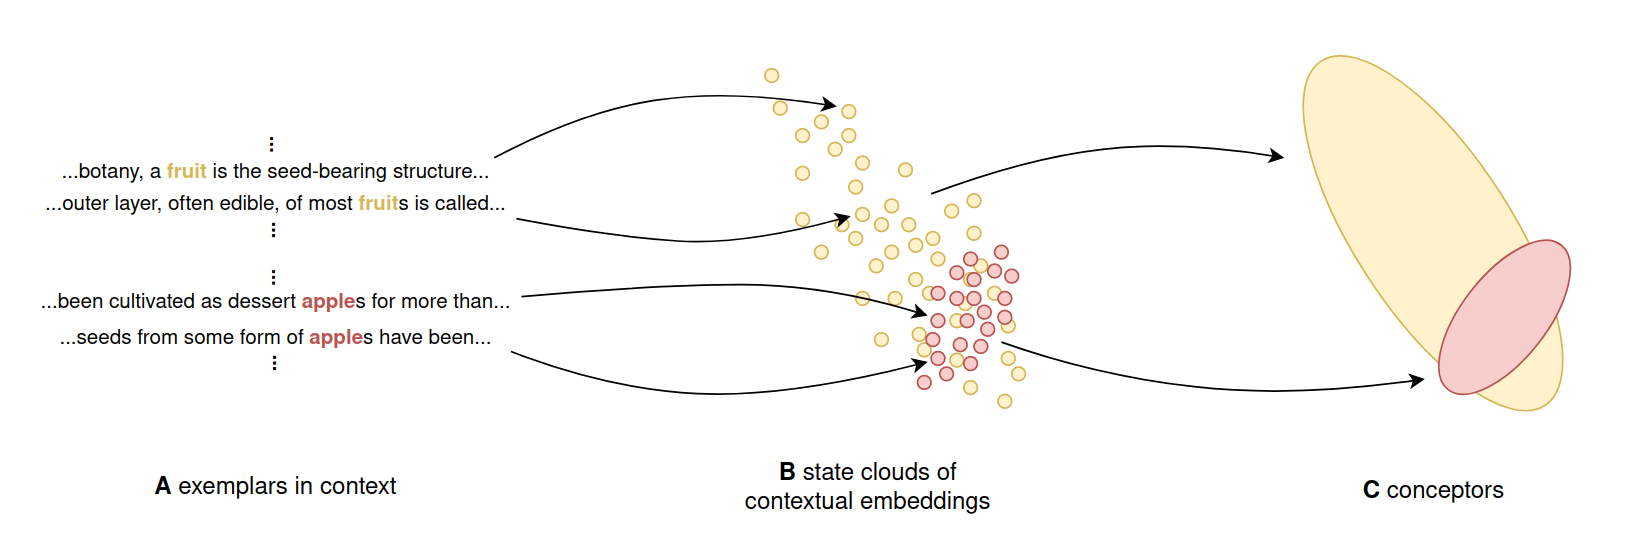
\includegraphics[width=\textwidth]{img/exemplars-conceptors.png}
    \caption{A: Exemplars are located and extracted together with their surrounding contexts. B: Each exemplar is encoded into a contextual embedding. Notably, the same symbol is encoded into different such embeddings based on context, resulting in a state cloud per symbol. C: Conceptors are derived from each state cloud as more compact representations.}\label{fig:exemplars-conceptors}
\end{figure*}

From each remaining state cloud representing the set of exemplars contained in the dataset, we obtain a conceptor \citep{jaeger_controlling_2017} (\ref{fig:exemplars-conceptors}). For completeness, a conceptor is a mathematical object which models the distribution of state cloud in the space it populates. However, conceptors do \textit{not} represent the \textit{density} of embeddings in space using a probability density function. Rather, a conceptor represents the orthogonal \textit{directions} across which the state cloud spreads most across space, together with the spread associated with each direction. This information can be compactly represented in a square matrix whose dimensionality matches the one of the space populated by the state cloud.

Both conceptors and Principal Component Analysis (PCA) make use of the correlation matrix of the state cloud. However, an additional parameter appears in the case of conceptors. Specifically, a conceptor also requires an aperture to be defined. The aperture $\alpha$ is a parameter which dictates the extent to which the shape of the state cloud is reflected in the associated conceptor object. For increasing aperture values, the conceptor matrix approaches the identity matrix. For decreasing aperture values, the conceptor matrix approaches the zero matrix.

Obtaining a conceptor from a state cloud is straight-forward and computationally cheap. Given the correlation matrix of the state cloud $R$ and a real value $\alpha$ specified for the aperture parameter, the conceptor matrix can be obtained through the following closed-form equation:$$C(R, \alpha) = R (R + \alpha^{-2} I)^{-1}.$$

In the present work, we only obtain conceptors from state clouds composed of contextual embeddings generated by the pretrained BERT model. Each state cloud contains contextual embeddings associated with one symbol composed of one or several tokens (e.g. "orange juice"), while each individual contextual embedding is associated with a specific exemplar. Given that we obtain conceptors from state clouds of BERT contextual embeddings, the dimensionality of the state cloud matches that of the embeddings, namely $$d_{BERT}=768.$$ We note that the interpretability technique we introduce does not require this specific dimensionality. Rather, the specific value of $d_{BERT}$ is only an artifact of the investigated model's architecture. It is likely that NSC could be applied with minimal modifications to state clouds of lower or higher dimensionality. In fact, some of the experiments used to introduce conceptors as mathematical objects make use of state clouds of only several dimensions.

Additionally, it is useful to note the large difference in terms of memory footprint observed between a state cloud of BERT embeddings and a conceptor matrix derived from it. A state cloud containing $n_{embs} = 10^6$ BERT embeddings of dimensionality $d_{BERT}=768$ naively requires $n_{embs} \cdot d_{BERT} = 7.68 * 10^8$ floating point values to fully represent. In contrast, the conceptor matrix obtained from the same state cloud, given a certain aperture, is a square matrix with $d_{BERT}$ rows and columns. Hence, it only needs $d_{BERT}^2 \approx 5.89 * 10^5$ floating point values to be represented. In this specific case, the conceptor represents the state cloud with an approximately $10^3$ times smaller memory footprint. Moreover, the memory footprint of the conceptor matrix is constant with respect to the cardinality of the state cloud. It is only the accuracy of representing the state cloud which increases with more samples in the form of new contextual embeddings, as the correlation matrix converges. The implication of this is that state clouds associated with symbols which have relatively high frequency in the auxiliary dataset get represented through conceptor matrices of the same size as those associated with symbols with relatively low frequency. That said, storing large numbers of conceptor matrices can still become expensive. In this case, a trade-off between numerical precision and memory footprint becomes relevant.

\subsection{Abstraction Ordering}

\begin{figure*}[h]
    \centering
    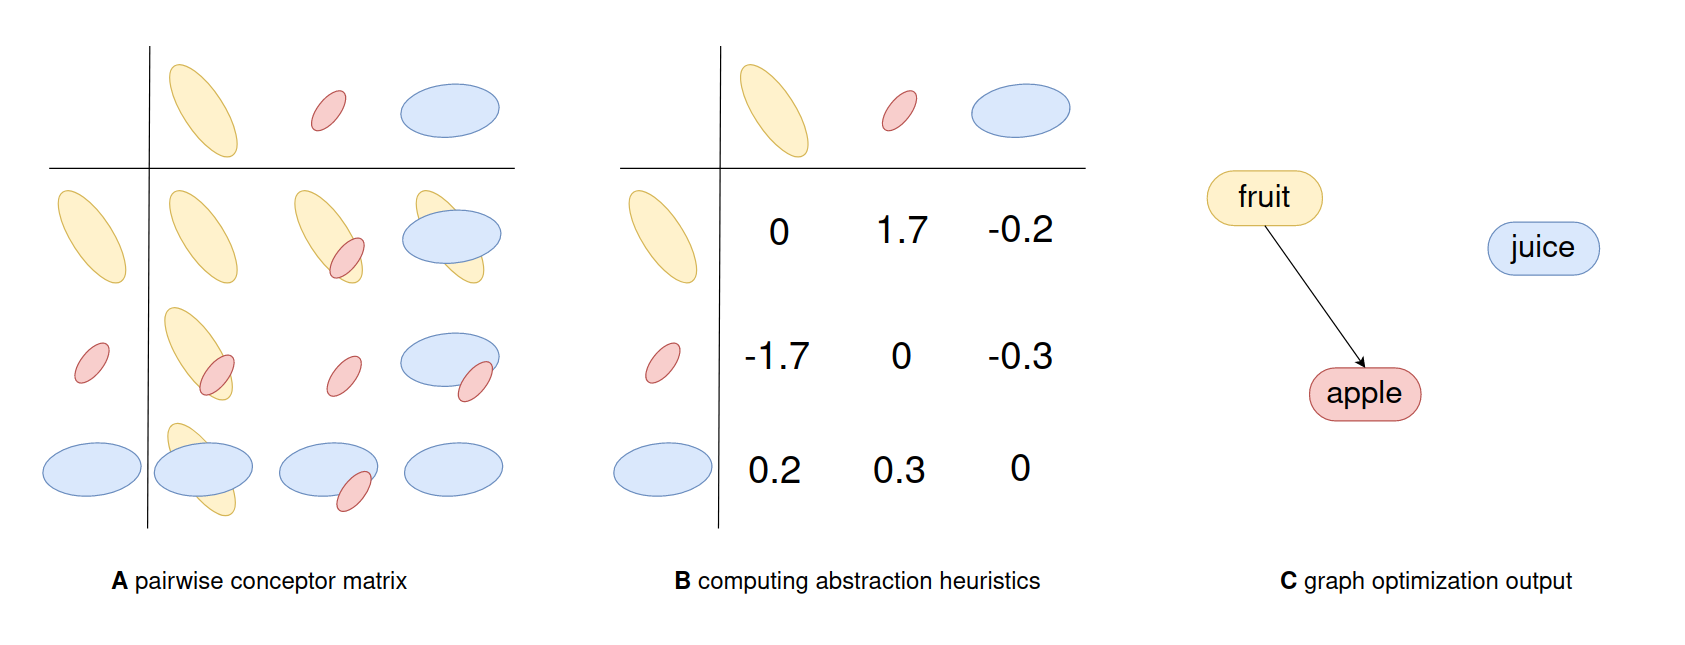
\includegraphics[width=\textwidth]{img/conceptors-graph.png}
    \caption{A: The matrix $D$ represents the pairwise relations of abstraction between conceptors. B: Matrix $D$ is populated using abstraction heuristics, where $D_{ij}$ approximates how much more abstract conceptor $C_i$ is with respect to conceptor $C_j$. C: The graph optimization process attempts to generate an ontology which is (1) faithful to the relations of abstraction identified previously, and (2) legible and sparse.}\label{fig:conceptors-graph}
\end{figure*}

For each pair of conceptors $(C_1, C_2)$ obtained from different state clouds of contextual embeddings, we attempt to estimate how they relate to each other in terms of abstraction (\ref{fig:conceptors-graph}). We aim to determine whether (1) $C_1$ represents a concept which is more abstract than the one represented by $C_2$ (e.g. "fruit" $>$ "apple"), whether (2) it is the other way around (e.g. "apple" $<$ "fruit"), or whether (3) the two concepts represented lack a meaningful abstraction ordering (e.g. "fruit" $<>$ "galaxy"). Ideally, we would only want the final knowledge graph generated by NSC to represent relations of decreasing abstraction by means of arcs (e.g. "fruit" $>$ "apple"). This would conceivably lead to a knowledge graph which approaches a hierarchical structure.

In its original formulation, abstraction ordering of conceptors has two important characteristics \citep{jaeger_controlling_2017}. First, prior art only describes the three mutually-exclusive cases above, with hard limits. $C_1$ is described to be more abstract than $C_2$ if and only if the difference matrix $C_1 - C_2$ is positive definite. Due to the symmetry of abstraction ordering, $C_2 > C_1$ if and only if the difference matrix $C_2 - C_1$ is positive definite. In the third case, the conceptor matrices are equal.

Unfortunately, real data is noisy, making it extremely unlikely that the unambigious criterion of positive definiteness ever holds for conceptors obtained from non-synthetic data (e.g. BERT contextual embeddings). Besides the inevitable aleatoric noise associated with non-synthetic data, abstraction ordering in its original formulation is also hindered by the cumulative error introduced by limited machine precision when dealing with floating point values. Approaches from numerical methods, however, might help mitigate the impact of this second source of noise.

Besides requiring standards of precision and signal-to-noise ratio which are non-trivial to attain in practice, abstraction ordering in its original formulation also happens to provide hard cut-offs. $C_1$ can be determined to be more abstract than $C_2$, less abstract, or equally abstract. In practice, a continuous signal representing \textit{how much} more abstract $C_1$ is compared to $C_2$ appears to be quite useful relative to the original ternary signal. In attempting to make use of an abstraction ordering signal which (1) is decently robust against the noise of real-world data, and (2) can be used to gauge the precise \textit{magnitude} of the abstraction difference, we introduce a heuristic. The design of this heuristic has been informed by the fact that symmetric positive definite matrices only have positive eigenvalues. This property has led to the idea of mean-pooling eigenvalues and using both the polarity and magnitude of the result as a proxy for abstraction ordering of two given conceptors.

Concretely, we estimate the abstraction ordering of $(C_1, C_2)$ by means of the following heuristic:$$f(C_1, C_2) = \frac{1}{d_{BERT}} \sum\limits_{i=1}^{d_{BERT}} \lambda_i(C_1 - C_2).$$ To unpack, we first substract one conceptor matrix from the other. Second, we compute the mean of the eigenvalues of the difference matrix, where $\lambda_i$ denotes the \textit{i'th} largest eigenvalue of said matrix. Intuitively, all eigenvalues of the difference matrix are positive if the first conceptor spatially engulfs the other, having higher spread than the second across all dimensions. In the context of this project, across all $d_{BERT} = 768$ dimensions. Conversely, all such eigenvalues are negative if the first conceptor is completely contained by the second across all dimensions. Inevitably, however, the two conceptors will exhibit one such relation across \textit{some} dimensions, while simultaneously exhibiting the opposite in other dimensions. Hence, we average the eigenvalues in an attempt to reach a "consensus opinion" as to how the two conceptors are related to each other in terms of abstraction.

\subsection{Graph Optimization}

Given the pairwise estimates of abstraction ordering computed before, we conduct a graph optimization process. All candidate graphs considered are directed ones, while nodes are identified with concepts, and arcs indicate meronymous relations of abstraction.

We attempt to solve the graph optimization task through the local search algorithm of simulated annealing (see Algorithm \ref{alg:gs}). Each candidate graph is represented through a Boolean adjacency matrix $A$. Specifically, $A^k$ denotes the adjacency matrix of the candidate graph considered at step $k$ of the graph optimization process. $A^k_{ij}$ is a Boolean value indicating whether concept $i$ links to concept $j$ in the associated candidate graph of step $k$. As an initial candidate graph, the optimization process starts with a fully-disconnected graph, where no concepts are related to each other. This is represented through an adjacency matrix full of null values, $A^0 = 0$. Then, we randomly sample a new graph proposal by randomly mutating the current graph in one location -- removing a previous arc or adding a new one. The acceptance probability is informed by a temperature schedule which linearly decreases from one to zero over the course of the optimization process, encouraging heavy exploration in the first epochs while using an increasingly conservative strategy towards the end.

The objective function which the search algorithm attempts to maximize is a linear combination of four different terms. Each term is a function of either or both (1) the adjacency matrix $A^k$ which is identified with the state of the graph optimization process in step $k$, and (2) the matrix $D$ containing pairwise estimates of abstract ordering. $D_{ij}$ denotes the numerical estimate of abstraction between conceptor $i$ and $j$. In other words, $$D_{ij} = f(C_i, C_j).$$ We note that the particular way $D_{ij}$ is related to $D_{ji}$ is determined by the choice numerical heuristic employed for abstraction ordering. In our case (i.e. mean of eigenvalues of difference matrix), $D_{ij} = -D_{ji}$, yet this is not necessarily the case when opting for other heuristics, as explored in the discussion (e.g. positive-negative eigenvalues ratio). Besides the two matrices just described which influence the objective function through the four terms whose description follows, the objective function is also influenced by the four coefficients which are used to weigh the four terms.

The first term is a function of both $A^k$ and $D$. It is equal to the mean of the abstraction ordering estimates represented in the candidate graph by means of arcs. From now on, we refer to this term as \textit{expressed abstraction} (EA). In case of a fully-disconnected graph (i.e. one in which no arc exists in the graph at all) represented by $A^k = 0$, $EA(A^k, D) = 0$. In contrast, in case of a fully-connected graph (i.e. one in which there exists an arc between any two nodes) represented by $A^k = 1$, $EA(A^k, D) = \frac{1}{n^2} \sum_{i=1}^{n} \sum_{j=1}^{n} D_{ij}.$ More generally, $$EA(A^k, D) = \frac{1}{n^2} \sum_{i=1}^{n} \sum_{j=1}^{n} A^k_{ij}D_{ij}.$$

In such case, $min(D) \leq EA(A^k, D) \leq max(D)$. This is the only among the four terms of the linear combination which indicates functional-groundedness, as it reflects the proportion of the abstraction identified in high-dimensional space which gets represented in the output knowledge graph.

The second term is only a function of $A^k$. It is equal to the proportion of arcs contained by the candidate graph represented by adjacency matrix $A^k$, relative to the maximum number of possible arcs $n^2$: $$AD(A^k) = \frac{1}{n^2} \sum_{i=1}^{n} \sum_{j=1}^{n} A^k_{ij}.$$ We refer to this term as \textit{arc density} (AD). In case of a fully-disconnected graph with $A^k = 0$, $AD(A^k) = 0$. In case of a fully-connected graph with $A^k = 1$, $AD(A^k) = 1$. In all other cases, $0 < AD(A^k) < 1$.

The third term is also only a function of $A^k$. It is equal to the mean difference between a node's children count (i.e. number of nodes connected via outbound arcs) and a target children count set in advance: $$CE(A^k) = \frac{1}{n} \sum_{i=1}^{n} \left|(\sum_{j=1}^{n}A^k_{ij}) - target\_children\right|.$$ We refer to this term as \textit{children error} (CE). In case of a graph with adjacency matrix $A^k$ in which every node only has children equal in count to $target\_children$, $CE(A^k)=0$. For all other graphs, $CE(A^k) > 0$.

The fourth and final term of the objective function is extremely similar to the previous one, yet it addresses the distribution of parent counts, rather than children counts. Concretely, it is equal to the mean difference between a node's parent count (i.e. number of nodes connected via inbound arcs) and a target parent count set in advance: $$PE(A^k) = \frac{1}{n} \sum_{j=1}^{n} \left|(\sum_{i=1}^{n}A^k_{ij}) - target\_parents\right|.$$ We refer to this term as \textit{parent error} (PE). In case of a graph with adjacency matrix $A^k$ in which every node only has parents equal in count to $target\_parents$, $PE(A^k)=0$. For all other graphs, $PE(A^k) > 0$.

We occasionally refer to arc density, children error, and parent error collectively as \textit{legibility terms}, because their sole role in the objective function of the graph optimization process is to directly influence the sparsity of the NSC output graph, as opposed to incentivizing the optimization process to adequately represent the relations of abstraction. The broader role of the legibility terms, as hinted at in the introduction, is to help generate sparse explanations which are cognitively ergonomic, or human-grounded, as phrased in the XAI literature \citep{madsen_post-hoc_2021}. In contrast, expressed abstraction is the only term of the objective function which incentivizes the adequate representation of abstraction ordering.

Besides the four terms which are functions of either or both $A^k$ and $D$, the objective function also contain four coefficients meant to influence the relative weight of each term. We denote these as $\alpha, \beta, \gamma$, and $\delta$ in order for the four terms. Given the four terms, the two additional targets for child and parent count, and the four weighing coefficients included in the linear combination, the objective function can finally be defined as:

\begin{align*}
     & score(A^k, D, target\_children, target\_parents) = \\
     & \alpha EA(A^k, D)                                  \\
     & - \beta AD(A^k)                                    \\
     & - \gamma CE(A^k, target\_children)                 \\
     & - \delta PE(A^k, target\_parents).
\end{align*}

The result of the graph search is the final output of NSC: a graph which indicates how the underlying DL model relates concepts by means of contextual embeddings. The final graph optimization step of NSC, which builds heavily on simulated annealing, has been summarized in pseudocode in Algorithm \ref{alg:gs}. Additionally, the whole NSC pipeline has been condensed in Algorithm \ref{alg:nsc} in order to offer an overview of the entire technique.

\begin{algorithm}[!tbp]
    \caption{Graph optimization in NSC}
    \label{alg:gs}
    \hspace*{\algorithmicindent} \textbf{Input}: $D$ \\
    \hspace*{\algorithmicindent} \textbf{Output}: $A^{opt}$
    \begin{algorithmic}
        \STATE $A^0 \Leftarrow 0 $ (fully-disconnected graph) \\
        \FOR{$k = 0$ to $epochs$}
        \STATE $T \Leftarrow 1 - \frac{k}{epochs}$ \\
        \STATE $A^{k+1} \Leftarrow neighbor(A^k)$ (one-arc change) \\
        \IF{$P_{acceptance}(score(D, A^k), score(D, A^{k+1}), T) \leq random(0, 1)$}
        \STATE $ A^{k+1} \Leftarrow A^{k}$
        \ENDIF
        \ENDFOR
        \STATE $A^{opt} \Leftarrow A^{epochs}$
    \end{algorithmic}
\end{algorithm}

\begin{algorithm}[!tbp]
    \caption{Nested State Clouds}
    \label{alg:nsc}
    \hspace*{\algorithmicindent} \textbf{Input}: $symbols$ \\
    \hspace*{\algorithmicindent} \textbf{Output}: $A^{opt}$
    \begin{algorithmic}
        \STATE $conceptors \Leftarrow \{\}$ \\
        \FOR{$s$ in $symbols$}
        \STATE $a \Leftarrow contexts(s)$ (list of contexts for exemplars) \\
        \STATE $b \Leftarrow cloud(a)$ (list of contextual embeddings of exemplars) \\
        \STATE $c \Leftarrow conceptor(b)$ (conceptor matrix obtained from state cloud)\\
        \STATE $conceptors \Leftarrow conceptors \cup \{c\}$
        \ENDFOR
        \FOR{$i, c_i$ in $conceptors$}
        \FOR{$j, c_j$ in $conceptors$}
        \STATE $D_{ij} \Leftarrow f(c_i, c_j)$
        \ENDFOR
        \ENDFOR
        \STATE $A^{opt} \Leftarrow graph\_optimization(D)$
    \end{algorithmic}
\end{algorithm}

In the context of the present work, we have manually specified values for the four coefficients of the linear combination which comprises the graph optimization objective: $\alpha, \beta, \gamma$, and $\delta$. Besides those, we have also manually specified values for the two hyperparameters related to local graph structure, $target\_children$ and $target\_parents$. However, a more robust approach to specifying the values of those six hyperparameters would be to conduct a hyperparameter search. Concretely, one might resort to searching for appropriate values for those six hyperparameters -- in addition to the number of graph optimization epochs, the temperature schedule, and the conceptor aperture -- which successfully recover some presupposed relations of abstraction between the concepts being related by means of the resulting knowledge graph. We leave that for future work and expand on the possibility in the discussion.